%
% File acl2019.tex
%
%% Based on the style files for ACL 2018, NAACL 2018/19, which were
%% Based on the style files for ACL-2015, with some improvements
%%  taken from the NAACL-2016 style
%% Based on the style files for ACL-2014, which were, in turn,
%% based on ACL-2013, ACL-2012, ACL-2011, ACL-2010, ACL-IJCNLP-2009,
%% EACL-2009, IJCNLP-2008...
%% Based on the style files for EACL 2006 by 
%%e.agirre@ehu.es or Sergi.Balari@uab.es
%% and that of ACL 08 by Joakim Nivre and Noah Smith

\documentclass[11pt,a4paper]{article}
\usepackage[hyperref]{acl2019}
\usepackage{times}
\usepackage{latexsym}
\usepackage{amsmath}
\usepackage{graphicx}
\usepackage{caption}
\usepackage{subcaption}
\usepackage{hyperref}

\usepackage{relsize}
\renewcommand*{\UrlFont}{\smaller\relax}


\DeclareMathOperator*{\argmax}{arg\,max}
\DeclareMathOperator*{\argmin}{arg\,min}
\usepackage{enumitem}


\usepackage{url}

\aclfinalcopy % Uncomment this line for the final submission
%\def\aclpaperid{***} %  Enter the acl Paper ID here

%\setlength\titlebox{5cm}
% You can expand the titlebox if you need extra space
% to show all the authors. Please do not make the titlebox
% smaller than 5cm (the original size); we will check this
% in the camera-ready version and ask you to change it back.
\newcommand\BibTeX{B\textsc{ib}\TeX}

\title{Concept Tagging for the Movie Domain by using Named Entity Recognition Tools.}

\author{Giovanni De Toni (197814) \\
  University of Trento \\ Via Sommarive, 9, 38123 Povo,Trento TN\\
  \texttt{giovanni.detoni@studenti.unitn.it}}

\date{}

\begin{document}
\maketitle

\begin{abstract}
This work focuses on the well-known task of concept tagging sentences.  It is the starting point for more complex techniques and it represents a relatively important challenge when building Spoken Language Understanding applications. This report details the realization of two SLU modules by using Named Entity Recognition tools for concept tagging sentences taken from the movie domain. We also show the performance obtained over various experiments.
\end{abstract}

\section{Introduction}
One of the first and most important of any NLP task is to analyze a given sentence to understand its underlying meaning. More specifically, we want to find the most likely interpretation which maps the utterance to given concepts. For instance, imagine we are using a vocal assistant to order something to eat (e.g., ``I would like a \textit{tortel de patate}\footnote{A typical northern-Italy dish.} to be delivered at \textit{Piazza Trento 1}, please"). Firstly, a machine needs to convert our utterances to a word representation. Secondly, it needs to assign a concept to each of the words it heard to understand correctly what we want (e.g., ``\textit{tortel de patate}" equals to a hypothetical ``FOOD" concept and ``\textit{Piazza Trento 1}" equals to the ``DELIVERY ADDRESS").
This basic operation is of utmost importance for all the applications which can be built upon this. For instance, the quality of your food assistant is dependent on the quality of this concept tagger. Imagine what could happen if the machine were to swap the delivery address with the requested food!.  
The scope of this project is to provide a simple concept-tagger by developing a Spoken Language Understanding Model applied to sentences in the movie domain by using statistical tools and Named Entity Recognition (NER) techniques.
The report is structured as follow: the first section defines more formally the problem statement, then we proceed with an analysis of the used dataset and with the description of the models employed. Ultimately, we discuss the experiments and the evaluation results while underlying the models' strengths and limitations.

 

\section{Problem Statement}
Given a sequence of tokens $<t_1, \ldots, t_n>$ and given a pool of concepts $<c_1, \ldots, c_m>$, we want to find the most likely assignment $<t_i, c_i>$ such that it maximizes the following probability:
\begin{equation}
c_1, \ldots, c_n = \argmax_{c_1, \ldots, c_n} P (c_1, \ldots, c_n | t_1, \ldots, t_n)
\label{frm:argmax}
\end{equation}
The previous formula can be made easier to compute thanks to the \textit{Markov assumption}. Namely, the probability of the $i$-th concept $c_i$ depends only on the $(i-1)$-th concept $c_{i-1}$ and the probability of the $i$-th token $t_i$ depends only on the $i$-th concept $c_i$. We can estimate the various parameters by \textit{Maximum Likelihood (MLE)}:
\begin{equation}
c_1, \ldots, c_n = \argmax_{c_1, \ldots, c_n} \prod_{i=1}^n P(t_i|c_i)P(c_i| c_{i-1})
\label{frm:argmax-markov-assumption}
\end{equation}
In the previous formula, $P(t_i|c_i) = \frac{C(c_i, t_i)}{C(c_i)}$ and $P(c_i|c_{i-1}) = \frac{C(c_{i-1}, c_i)}{C(c_i)}$ (where $C(x)$ counts the occurrences of $x$ inside the given dataset). 

\begin{table*}
    \begin{subtable}{.5\linewidth}
		\centering
\begin{tabular}{|l|l|}
\hline
\multicolumn{2}{|l|}{\textbf{NL2SparQL4NLU.train.conll.txt}} \\ \hline
\textit{\# of lines}									& 24791 \\ \hline
\textit{\# of sentences}                             & 3338 \\ \hline
\textit{Dictionary size (\# unique tokens)}                         & 1728 \\ \hline
\end{tabular}
\caption{Train dataset.}
\end{subtable}%	
\begin{subtable}{.5\linewidth}
\centering
\begin{tabular}{|l|l|}
\hline
\multicolumn{2}{|l|}{\textbf{NL2SparQL4NLU.test.conll.txt}} \\ \hline
\textit{\# of lines}									& 8201 \\ \hline
\textit{\# of sentences}                             & 1084 \\ \hline
\textit{Dictionary size (\# unique tokens)}                         & 1039 \\ \hline
\end{tabular}
\caption{Test dataset.}
\end{subtable}
\caption{Brief description of the content of the dataset used.}
\label{tab:test-dataset-description}
\end{table*} 

\section{Data Analysis}

We used the dataset called \textit{NL2SparQL4NLU}\footnote{\url{https://github.com/esrel/NL2SparQL4NLU}} \citep{Chen2014DerivingLR, gobbi2018concept}. It contains several English sentences related to the movie domain. This work used only the ``*.conll.txt" files. More specifically, one for training the language model and one for testing it. Each file is written using the token-per-line \textit{CONLL} format with tokens and NLU concept tags. Table \ref{tab:test-dataset-description} provides a general description of the two files. The average length of the sentences is around 6.42 and 6.52 for the train and test dataset respectively. The \textit{OOV rate} for the tokens between the train and the test dataset is around $0.24\%$.


Figure \ref{fig:concept-distribution} shows the distribution of the various concepts. 
There are 23 distinct concepts which define 43 tags in IOB tagging format. We noted that the ``O" concept represents the $70\%$ of the dataset, which poses a significant problem for the tagging procedure. The concept graphs do not show the ``O" concept percentage to make it easier to visualize the distribution of the other concepts. It is possible to see how the \textit{movie.name} concept is one of the most common, followed by \textit{actor.name} and \textit{director.name}.


Moreover, both the train and test set contains concepts which are not present in the other dataset (and vice-versa). The train dataset contains \textit{person.nationality} (2 occurrences) and \textit{movie.description} (2 occurrences) which are not present in the test set. The test dataset contains the concept \textit{movie.type} which is missing from the training dataset (4 occurrences). These again could cause mistagging issues and therefore lower the final performance of the SLU model. 
As a final note, there are also
some tokens which are the results of misspelling errors (e.g., ``dispaly", ``Scorcese") which could lead to other tagging inaccuracies.



\section{Models}

\begin{figure}[b!]
\centering
	\includegraphics[width=1\linewidth]{img/entity}
	\caption{Example of named entity recognition. For instance, the ``\textit{ed harris}" tokens were recognized as a PERSON while ``\textit{thirteen}" was recognized as number.}
	\label{fig:entity-recognition}
\end{figure}

In this work, we devised and evaluated two separated SLU models. 
The first SLU model was trained by using directly the dataset provided (without modifications) and it 
implements Formula \ref{frm:argmax-markov-assumption}. 
This first model was used as the baseline. The second model uses named entity recognition tools which convert certain token(s) to an entity definition before training the complete language model. See Figure \ref{fig:entity-recognition} for an example of named entity recognition. These entity definitions replace the previous tokens. We chose two external libraries which provides two pre-trained NER classifier: \textbf{NLTK}\footnote{\url{https://www.nltk.org/}} and \textbf{spaCy} \footnote{\url{https://spacy.io/}}. 
We performed these improvements to mitigate some ambiguity and variability issues which are presents in the dataset. 
More specifically, some tokens refer to the same entity 
and the same concept while they may have different values 
(e.g., ``\textit{nick fury}" and ``\textit{robin}" are both 
``\textit{persons}" (entity) and ``\textit{character names}" (concept), even if  they have different tokens). 
As the dataset analysis showed us, the majority of the concepts are equal to ``\textit{O}" which is not informative enough. A possible solution already used in the literature is to substitute each occurrence of the  ``O" concept with another value. We tried three possible substitution policies. We used: 
directly the corresponding \textbf{token value}, the \textbf{token stem} and the \textbf{token lemma}.
 


\begin{figure*}
	\begin{subfigure}[b]{0.5\linewidth}
		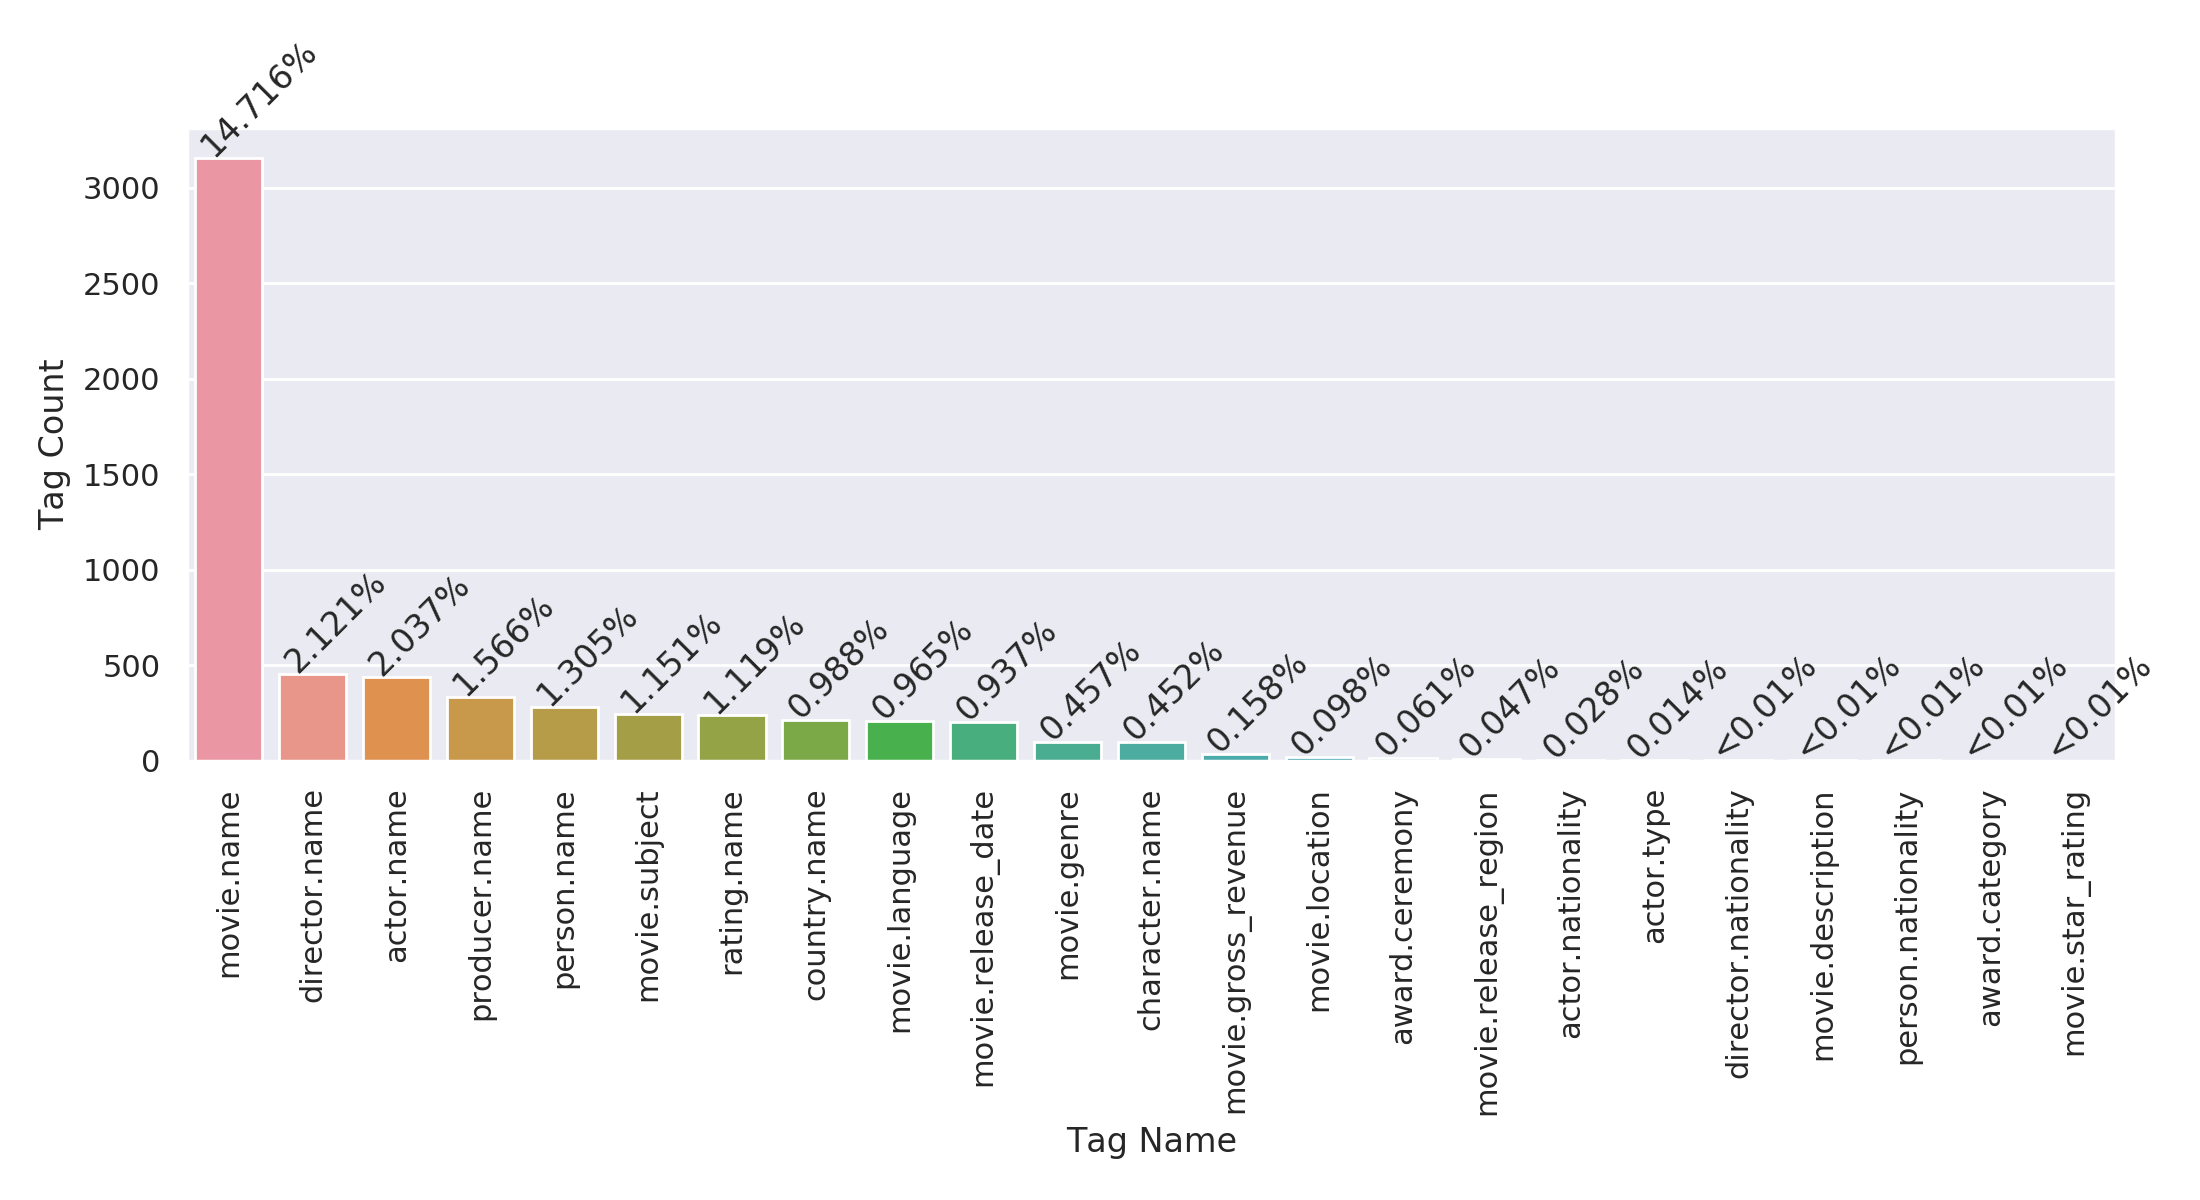
\includegraphics[width=\linewidth]{img/train-concepts-distribution}
		\caption{Train dataset.}
	\end{subfigure}
	\begin{subfigure}[b]{0.5\linewidth}
	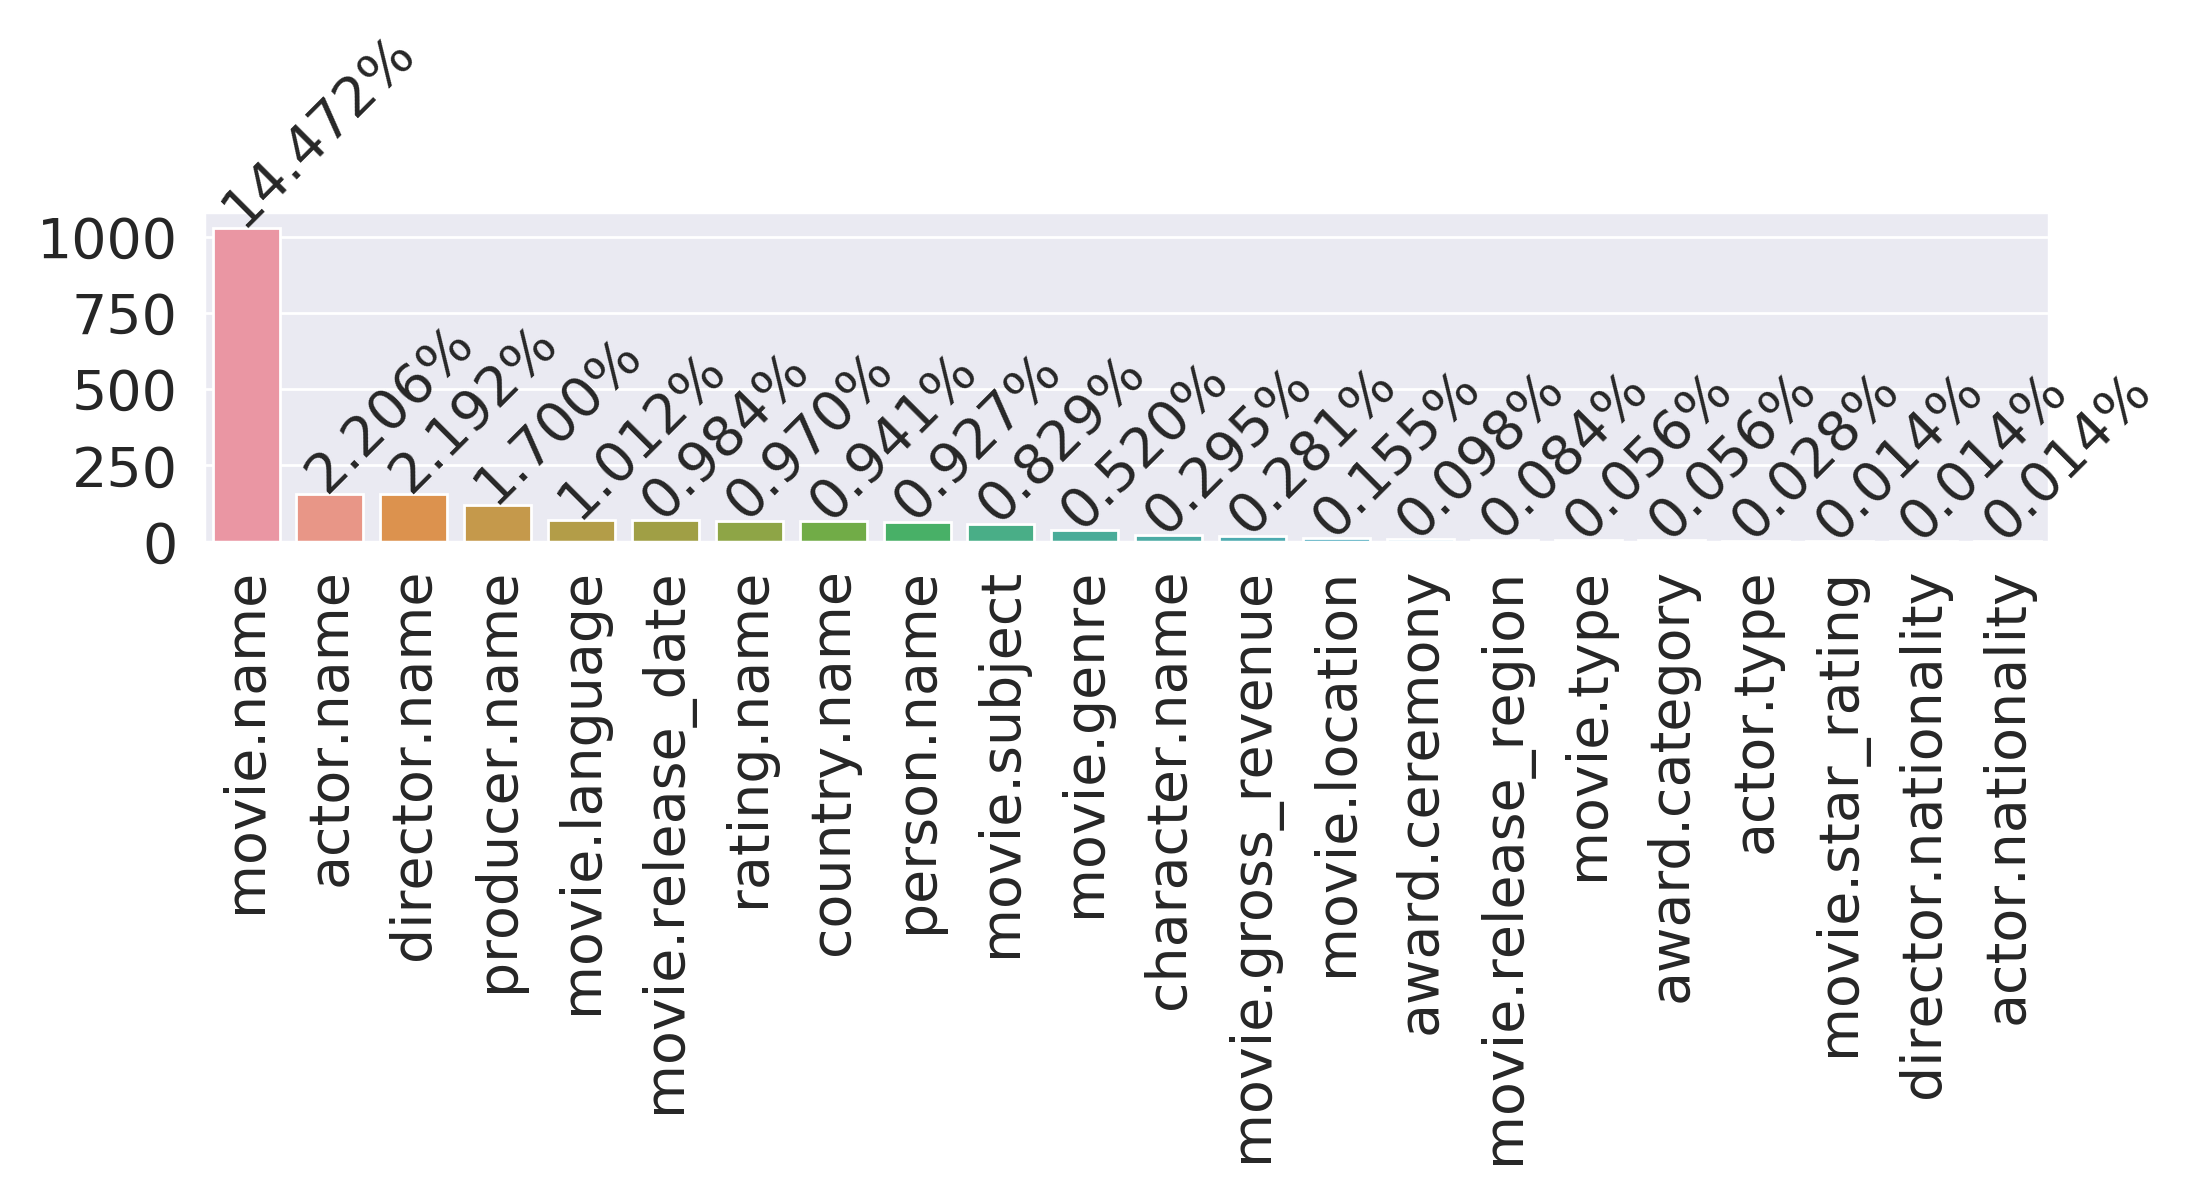
\includegraphics[width=\textwidth]{img/test-concepts-distribution}
	\caption{Test dataset.}
	\end{subfigure}
	\caption{Distributions of the various concepts in the train and test datasets. The ``O" concept was removed to make it easier to understand the weight of the other concepts.}
	\label{fig:concept-distribution}
\end{figure*}

\subsection{Spoken Language Understanding Pipeline}

The entire SLU pipeline of both models includes two main components: the \textit{Concept Tagger (WFST)} and the \textit{Language Model (LM)}. Moreover, the \textit{Named Entity Recognition Classifier} can be optionally used before building the WFST and the LM. 


\subsubsection{NER Classifier}

The \textit{Named Entity Recognition classifier} was used to convert certain tokens (or group of tokens) into \textit{entities}. After applying the classifier and after having removed the possible duplicates entities (e.g., \textit{ed harris} is resolved into \textit{PERSON PERSON} instead of just one entity \textit{PERSON}), we obtained a final phrase which was to build the SLU model. Below we show an example of the process:

\begin{enumerate}[noitemsep]
\item \textit{what year was ed harris in in apollo thirteen}
\item \textit{DATE was PERSON in in apollo CARDINAL}
\item \textit{O O B-actor.name O O B-movie.name I-movie.name}
\end{enumerate}

The first phrase is the original. The second represents the ``translation" made by the NER and the third represents the final concepts. Apart from the double ``\textit{in}", we can already seen the limits of this approach (e.g. \textit{apollo thirteen} is not recognized as a definite entity). 

\subsubsection{Concept Tagger (WFST)}
It is a transducer which encodes the probability $P(t_i|c_i) = \frac{C(c_i, t_i)}{C(c_i)}$. The probability (score) is the weight given to the transition from the given token to the concept (see Figure \ref{fig:transducer}). To prevent numerical stability issues, the negative log was applied to the probability. Therefore, the weights assigned to the transitions are computed by using $-log(P(t_i|c_i))$. An additional token called $<$\textit{unk}$>$ was added to the transducer to account for Out of Vocabulary words (namely, tokens which are present in the test dataset, but not in the lexicon). Moreover, for each of the possible concepts $c_i$, a transition $<$\textit{unk}$>$:$c_i$ was added with a score of $\frac{1}{\#concepts}$ (this means that each unknown token has an equal probability of ``representing" each concept). 

\begin{figure}[b!]
	\centering
	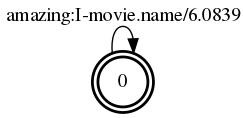
\includegraphics[width=0.5\linewidth]{img/pos-tagger}
	\caption{Example of a possible transducer in which the token \textit{amazing} is mapped to the concept \textit{I-movie.name} with an associated transition score.}
	\label{fig:transducer}
\end{figure}

\subsection{Language Model (LM)}
It is a transducer which encodes the probability $P(c_i|c_{i-1}) = \frac{C(c_{i-1}, c_i)}{C(c_i)}$, which means finding a concept $c_i$ conditioned on having seen concept $c_{i-1}$. 

\subsection{Final SLU Model}

The previous components need to be composed together with the sentence we want to tag to be used.
\begin{equation}
\lambda_{CT} = \lambda_{sentence} \circ \lambda_{WFST} \circ \lambda_{LM}
\end{equation}
Then, we need to find the path which minimizes the cost within the final transducer (since we are using $-log()$ to compute the weights, minimizing the path cost is the equivalent of maximizing the probability of that tagging sequence). This final operation corresponds to computing the equation shown in Formula \ref{frm:argmax-markov-assumption}.


\begin{table*}[th!]
\centering
\caption{Best K-fold cross-validation results ($K=3$). The bold values indicate the best score. The underlined values indicate the overall best hyperparameters combination. The baseline is shown on the first line from the top.}
\label{tab:eval-resuts}
\begin{tabular}{llllll}
\textbf{Ngram Size} & \textbf{Smoothing} & \textbf{Pruning} & \textbf{Replace O} & \textbf{K-fold F1 Score} & \textbf{K-fold F1 Score (spaCy)} \\ \hline
\textit{4} & \textit{kneser\_ney} & \textit{5} & \textit{keep} & \textit{75.0467} & \textit{74.4367} \\ \hline
4 & kneser\_ney & 5 & lemma & \textbf{83.45} & 83.2167 \\
4 & kneser\_ney & 5 & stem & \textbf{83.6067} & 83.5033 \\
\underline{4} & \underline{kneser\_ney} & \underline{5} & \underline{token} & \textbf{83.73} & 83.5467 \\
4 & witten\_bell & 5 & token & 83.3633 & \textbf{83.4567} \\
4 & katz & 5 & stem & 82.8733 & \textbf{83.1033}
\end{tabular}
\end{table*}

\section{Experiments}

We run several experiments to assess the quality of 
the SLU models. For each provided solution, we performed an \textbf{extensive hyperparameters search} by trying several \textbf{smoothing techniques}, \textbf{ngram sizes}, \textbf{pruning frequencies} and the ``O" concept replacement methods. As a metric, we tried to find the solution which maximizes the \textit{F1-score} over the test set. Each solution was evaluated by using \textit{K-fold cross-validation} ($k=3$) and the best result was then recorded. Firstly, we evaluated the SLU model based directly on the given dataset without any further improvements. The best combination was then used as a baseline. Secondly, we evaluated the NER SLU model. 
The code employed for the project is publicy available on Github\footnote{\url{https://github.com/geektoni/concept\_tagging\_NLP}}. OpenFST \footnote{\url{http://www.openfst.org/}} and OpenGRM\footnote{\url{http://www.opengrm.org/}} libraries were used to build the WFST and the language model.
The experiments were run on an 8th-core Intel i7 CPU with 16GB of RAM. 



\section{Results}

Table \ref{tab:eval-resuts} shows the best results over all the hyperparameters combinations tested. We were able to increase the performances of around 8\% from the baseline by replacing the ``O" concepts with either the \textbf{stem}/\textbf{lemma} of the token or the token itself as expected.
However, \textbf{we did not notice any significative improvements by using the NER classifiers} (apart from a reduction of the \textit{perplexity} from 2492.06 to 1815.36).  We were able to improve the precision and recall of certain concepts when using an NER classifier (e.g., \textit{movie.gross\_revenue}, \textit{movie.release\_date} or \textit{movie.language}), but we also reduced the precision and recall of other concepts with a higher distribution (e.g., \textit{movie.name} or \textit{producer.name}), thus lowering the overall performances. The NER SLU model performs a little better when using the Witten-Bell/Katz smoothing method, but we did not gain any important improvement. We also discovered that \textbf{the spaCy NER classifier performs better than the NLTK NER classifier}. 
Therefore, the performance with NLTK was not reported in this report since they were almost similar to the non-NER SLU results.

We think that adding the spaCy NER classifier does not improve the performances mainly because it was trained on the OntoNotes dataset \footnote{\url{https://catalog.ldc.upenn.edu/LDC2013T19}} which is a general source for annotated text and \textbf{it is not specific for the movie domain}. Therefore, the entities used are quite general (e.g., PERSON instead of ACTOR or DIRECTOR). This caused some errors when doing named entity resolution (e.g., ``\textit{apollo 13}" is the title of a film, but just 13 was recognized as a CARDINAL entity, while both the tokens should have been recognized).
Furthermore, the original dataset had some issues regarding its concepts definition. Some of them have a very similar meaning and they represent the same entity in the end. For example, \textit{movie.location} and \textit{move.country} resolves into GPE (GeoPolitical Entity). Therefore, it happened that some tokens were tagged as \textit{movie.location} instead of \textit{movie.country}. 
 
One possible solution would be to build a \textbf{custom Named Entity Recognition model} specifically trained on the NL2SparQL4NLU dataset such to categorize more efficiently the various tokens. Moreover, more complex models \citep{gobbi2018concept} could be explored (e.g., deep neural networks)  and we could try to devise better features from the training dataset.

\bibliography{acl2019}
\bibliographystyle{acl_natbib}

\end{document}
